\documentclass{article}
\usepackage[utf8]{inputenc}
\usepackage[portuges]{babel}
\usepackage{ntheorem}
\usepackage{amsfonts}
\usepackage{amsmath}
\usepackage{amssymb}
\usepackage{diffcoeff}

%\usepackage[margin=1.5in]{geometry}
\usepackage{multicol}
\theorembodyfont{\upshape}
\theoremseparator{.}
\newtheorem{ex}{Exercício}[section]

\usepackage{enumitem}
\setlist[enumerate, 1]{label=\alph*)}

\usepackage{listings}
\lstset{basicstyle=\ttfamily,mathescape,keepspaces,tabsize=2,
literate=
  {á}{{\'a}}1
  {à}{{\`a}}1
  {ã}{{\~a}}1
  {é}{{\'e}}1
  {ê}{{\^e}}1
  {í}{{\'i}}1
  {ó}{{\'o}}1
  {ú}{{\'u}}1
  {ç}{{\c{c}}}1}
\usepackage{graphicx}
\usepackage{url}
\usepackage{hyperref}

\title{Mini-Projetos de ME}
\author{}
\date{}
\setlength{\parindent}{0pt}
\newcommand{\Z}{\mathbb{Z}}
\newcommand{\R}{\mathbb{R}}
\newcommand{\N}{\mathbb{N}}
\newcommand{\Q}{\mathbb{Q}}

\begin{document}

\section{Aproximar $\pi$}

Objetivo: Aproximar numericamente $\pi$ de diversas formas diferentes.

Desafio: Calcular $\pi$ eficientemente com a maior precisão possível.

Nota: Este exercício fica mais fácil se permitires o cálculo de funções trigonométricas, e.g. basta calcular $\pi = 2 \mathop{\mathtt{arctan}}(\sqrt2 / 2)$. Logo, tenta evitar o seu uso se conseguires.

Os seguintes exercícios representam algumas formas sugeridas de aproximar $\pi$, mas poderás passar as que achares desinteressantes à frente, e se te ocorrer uma forma nova és bem-vindo a experimentar!

\begin{ex}
Calcula $\pi$ como a área do círculo de raio 1 das seguintes formas:
\begin{enumerate}
\item Cobre o quadrado $[-1,1]\times[-1,1]$ por uma grelha uniforme de $N^2$ pontos e conta quantos pontos estão dentro do círculo.

\item (Método de Monte Carlo) Em vez de uma grelha uniforme, gera agora $N$ pontos aleatórios no quadrado e relaciona a percentagem deles que calha dentro do quadrado com $\pi$.
\end{enumerate}
\end{ex}

\begin{ex}
Calcula $\pi$ como metade do comprimento da circunferência, partindo a circunferência em segmentos de reta e somando os seus comprimentos.

Nota: Poderias tentar parametrizar a circunferência como $(\cos\theta, \sin\theta)$, mas isso requer fazer variar o $\theta$ entre 0 e $2\pi$, o que requer já saberes o valor de $\pi$...
\end{ex}

\begin{ex}
Os seguintes métodos têm um benefício em relação aos anteriores: para além de aproximar $\pi$, permitem-te quantificar o erro, dando-te uma estimativa por baixo e outra por cima.

Para facilitar as contas nos seguintes exercícios, poderá ser conveniente olhares apenas para o primeiro quadrante.

\begin{enumerate}
\item Divide o quadrado uniformemente em $N^2$ quadrados. Conta quantos destes quadrados estão integralmente dentro do círculo, e quais destes estão fora. Então, uma estimativa por baixo de $\pi$ é dada pela área dos quadrados que estão dentro do círculo, e uma estimativa por cima é dada pela área dos que não estão totalmente fora.

\item O algoritmo anterior tem bastante desperdício. Considera a seguinte forma recursiva de o optimizar:
\begin{itemize}
\item Parte o quadrado em quatro
\item Vê quantos pedaços estão inteiramente dentro do círculo, e quantos estão fora
\item Repete recursivamente, apenas nos quadrados que não estão totalmente dentro nem fora.
\end{itemize}

(Não te esqueças de adicionar uma condição de paragem, caso contrário mandas o computador abaixo!)
\end{enumerate}
\end{ex}

\section{Aproximação por polinómios}

[Este exercício requer conhecimento básico de integrais.]

Uma estratégia comum de aproximação de funções por polinómios é o uso de polinómios de Taylor. Neste exercício vais aprender outra forma.

Objetivo: Aproximar uma função (digamos, o seno) por polinómios de grau fixo $k$.

Ideia: Usar projeções ortogonais de Álgebra Linear. Podemos ver a coleção das funções contínuas no intervalo $[0,2\pi]$, chamado $C[0,2\pi]$ como um espaço vetorial com um produto interno (detalhes abaixo). Por sua vez, podemos ver a coleção de polinómios reais de grau $k$ ou abaixo, digamos $P_k$, como um subespaço linear de $C[0,2\pi]$. Assim sendo, dada uma função $f \in C[0,2\pi]$ podemos considerar a projeção ortogonal de $f$ em $P_k$ como sendo a `melhor' aproximaçao de $f$ por um polinómio de grau $k$ ou menor.

\begin{ex}
Considera o seguinte produto interno em $C[0,2\pi]$:\footnote{Não tens de justificar que é um produto interno. Nota que isto é a generalização natural da norma euclideana em $\R^n$, dada por $\langle u, v \rangle = \sum u_i v_i$; substituiu-se somente o somatório por um integral. Este produto interno em $C[0,2\pi]$ é normalmente chamado o produto interno $L^2$.}

\[\langle u, v \rangle = \int_0^{2\pi} u(t) v(t) \dl t.\]

Calcula a projeção da função $\sin$ em $P_k$. Experimenta também com outras funções e intervalos.
\end{ex}

\section{Desenhar Fractais}

Um fractal que poderás conhecer é a chamada `Curva do Dragão'. Encontra-se abaixo um algoritmo em pseudo-código para o desenhar. Tenta traduzir este algoritmo para código \textit{Mathematica}. Os seguintes comandos poderão ser úteis: \texttt{RotationMatrix}, \texttt{Dot} (para multiplicar uma matriz por um vetor), \texttt{Join}, \texttt{Nest}.

\begin{lstlisting}
Começar com um segmento de reta $S_0$
Construir a $n+1$-ésima iterada $S_{n+1}$ a partir de $S_n$:
	Seja $p$ o ponto final de $S_n$,
	Rodar $S_n$ por $\pi/2$ em torno de $p$. Chamar a isso $S'_n$.
	A curva $S_{n+1}$ é dada pela concatenação de $S_n$ com $S'_n$.
\end{lstlisting}

\begin{figure}
\centering
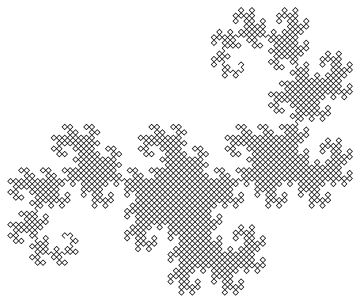
\includegraphics[width=6cm]{dragon.png}
\caption{A curva do dragão (iterada 13)}
\end{figure}
\begin{figure}
\centering
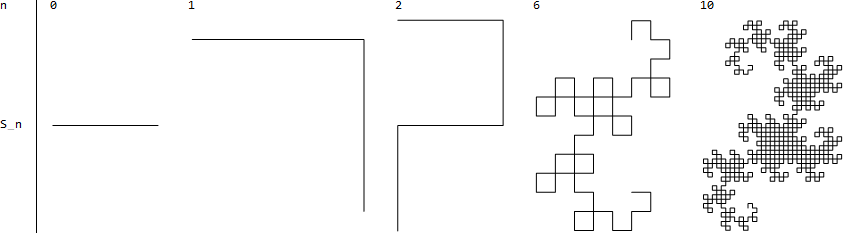
\includegraphics[width=\textwidth]{dragontable.png}
\caption{Algumas iteradas da curva do dragão}
\end{figure}

\begin{ex}
Desenha a Curva do Dragão.

Vê tambêm a página da Wikipedia: \url{https://en.wikipedia.org/wiki/Dragon_curve}
\end{ex}

\begin{ex}
Eis alguns outros exemplos de fractais que poderás desenhar:

\begin{enumerate}
\item Árvore fractal: \url{https://en.wikipedia.org/wiki/Fractal_canopy}

Para construir uma árvore fractal: Começa com um segmento de reta vertical $S_0$. Para construir $S_{n+1}$, faz duas cópias re-escaladas e rodadas de $S_n$, e cola-as ao extremo superior de $S_0$.

Experimenta usar re-escalamentos e rotações diferentes ou aleatórias.

\item \url{https://en.wikipedia.org/wiki/Barnsley_fern}

\item Curvas de Koch-Peano e de deRham: \url{https://en.wikipedia.org/wiki/De_Rham_curve}
\end{enumerate}
\end{ex}




\end{document}